% Options for packages loaded elsewhere
\PassOptionsToPackage{unicode}{hyperref}
\PassOptionsToPackage{hyphens}{url}
\PassOptionsToPackage{dvipsnames,svgnames,x11names}{xcolor}
%
\documentclass[
  super,
  preprint,
  3p]{elsarticle}

\usepackage{amsmath,amssymb}
\usepackage{iftex}
\ifPDFTeX
  \usepackage[T1]{fontenc}
  \usepackage[utf8]{inputenc}
  \usepackage{textcomp} % provide euro and other symbols
\else % if luatex or xetex
  \usepackage{unicode-math}
  \defaultfontfeatures{Scale=MatchLowercase}
  \defaultfontfeatures[\rmfamily]{Ligatures=TeX,Scale=1}
\fi
\usepackage{lmodern}
\ifPDFTeX\else  
    % xetex/luatex font selection
\fi
% Use upquote if available, for straight quotes in verbatim environments
\IfFileExists{upquote.sty}{\usepackage{upquote}}{}
\IfFileExists{microtype.sty}{% use microtype if available
  \usepackage[]{microtype}
  \UseMicrotypeSet[protrusion]{basicmath} % disable protrusion for tt fonts
}{}
\makeatletter
\@ifundefined{KOMAClassName}{% if non-KOMA class
  \IfFileExists{parskip.sty}{%
    \usepackage{parskip}
  }{% else
    \setlength{\parindent}{0pt}
    \setlength{\parskip}{6pt plus 2pt minus 1pt}}
}{% if KOMA class
  \KOMAoptions{parskip=half}}
\makeatother
\usepackage{xcolor}
\usepackage{soul}
\setlength{\emergencystretch}{3em} % prevent overfull lines
\setcounter{secnumdepth}{5}
% Make \paragraph and \subparagraph free-standing
\ifx\paragraph\undefined\else
  \let\oldparagraph\paragraph
  \renewcommand{\paragraph}[1]{\oldparagraph{#1}\mbox{}}
\fi
\ifx\subparagraph\undefined\else
  \let\oldsubparagraph\subparagraph
  \renewcommand{\subparagraph}[1]{\oldsubparagraph{#1}\mbox{}}
\fi


\providecommand{\tightlist}{%
  \setlength{\itemsep}{0pt}\setlength{\parskip}{0pt}}\usepackage{longtable,booktabs,array}
\usepackage{calc} % for calculating minipage widths
% Correct order of tables after \paragraph or \subparagraph
\usepackage{etoolbox}
\makeatletter
\patchcmd\longtable{\par}{\if@noskipsec\mbox{}\fi\par}{}{}
\makeatother
% Allow footnotes in longtable head/foot
\IfFileExists{footnotehyper.sty}{\usepackage{footnotehyper}}{\usepackage{footnote}}
\makesavenoteenv{longtable}
\usepackage{graphicx}
\makeatletter
\def\maxwidth{\ifdim\Gin@nat@width>\linewidth\linewidth\else\Gin@nat@width\fi}
\def\maxheight{\ifdim\Gin@nat@height>\textheight\textheight\else\Gin@nat@height\fi}
\makeatother
% Scale images if necessary, so that they will not overflow the page
% margins by default, and it is still possible to overwrite the defaults
% using explicit options in \includegraphics[width, height, ...]{}
\setkeys{Gin}{width=\maxwidth,height=\maxheight,keepaspectratio}
% Set default figure placement to htbp
\makeatletter
\def\fps@figure{htbp}
\makeatother

\usepackage{booktabs}
\usepackage{caption}
\usepackage{longtable}
\usepackage{lineno}\linenumbers
\makeatletter
\makeatother
\makeatletter
\makeatother
\makeatletter
\@ifpackageloaded{caption}{}{\usepackage{caption}}
\AtBeginDocument{%
\ifdefined\contentsname
  \renewcommand*\contentsname{Table of contents}
\else
  \newcommand\contentsname{Table of contents}
\fi
\ifdefined\listfigurename
  \renewcommand*\listfigurename{List of Figures}
\else
  \newcommand\listfigurename{List of Figures}
\fi
\ifdefined\listtablename
  \renewcommand*\listtablename{List of Tables}
\else
  \newcommand\listtablename{List of Tables}
\fi
\ifdefined\figurename
  \renewcommand*\figurename{Figure}
\else
  \newcommand\figurename{Figure}
\fi
\ifdefined\tablename
  \renewcommand*\tablename{Table}
\else
  \newcommand\tablename{Table}
\fi
}
\@ifpackageloaded{float}{}{\usepackage{float}}
\floatstyle{ruled}
\@ifundefined{c@chapter}{\newfloat{codelisting}{h}{lop}}{\newfloat{codelisting}{h}{lop}[chapter]}
\floatname{codelisting}{Listing}
\newcommand*\listoflistings{\listof{codelisting}{List of Listings}}
\makeatother
\makeatletter
\@ifpackageloaded{caption}{}{\usepackage{caption}}
\@ifpackageloaded{subcaption}{}{\usepackage{subcaption}}
\makeatother
\makeatletter
\@ifpackageloaded{tcolorbox}{}{\usepackage[skins,breakable]{tcolorbox}}
\makeatother
\makeatletter
\@ifundefined{shadecolor}{\definecolor{shadecolor}{rgb}{.97, .97, .97}}
\makeatother
\makeatletter
\makeatother
\makeatletter
\makeatother
\journal{npj Digital Medicine}
\ifLuaTeX
  \usepackage{selnolig}  % disable illegal ligatures
\fi
\usepackage[]{natbib}
\bibliographystyle{elsarticle-num}
\IfFileExists{bookmark.sty}{\usepackage{bookmark}}{\usepackage{hyperref}}
\IfFileExists{xurl.sty}{\usepackage{xurl}}{} % add URL line breaks if available
\urlstyle{same} % disable monospaced font for URLs
\hypersetup{
  pdftitle={Estimating Sleep Quality Metrics Using Free-Living Accelerometer Data From Thigh-Worn Devices in Comparison to an EEG-Based Sleep Tracking Device},
  pdfauthor={Esben Høegholm Lykke; Jan Christian Brønd},
  pdfkeywords={Sleep, Accelerometry, EEG, Machine learning, Sleep
quality metrics},
  colorlinks=true,
  linkcolor={blue},
  filecolor={Maroon},
  citecolor={Blue},
  urlcolor={Blue},
  pdfcreator={LaTeX via pandoc}}

\setlength{\parindent}{6pt}
\begin{document}

\begin{frontmatter}
\title{Estimating Sleep Quality Metrics Using Free-Living Accelerometer
Data From Thigh-Worn Devices in Comparison to an EEG-Based Sleep
Tracking Device}
\author[1]{Esben Høegholm Lykke%
\corref{cor1}%
}
 \ead{eskovgaard@health.sdu.dk} 
\author[1]{Jan Christian Brønd%
%
}
 \ead{jbrond@health.sdu.dk} 

\affiliation[1]{organization={University of Southern Denmark, Department
of Sports Science and Clinical Biomechanics},addressline={Campusvej
55},city={Odense},postcode={5230},postcodesep={}}

\cortext[cor1]{Corresponding author}


        
\begin{abstract}
LÆS IKKE! Det er volapyk på latin. Lorem ipsum dolor sit amet,
consectetur adipiscing elit. Suspendisse vitae dictum eros, ullamcorper
elementum orci. Sed laoreet nulla neque, pulvinar fermentum mi iaculis
at. Nulla ultricies nibh sit amet vestibulum rutrum. Nam pharetra nisl
sed ipsum maximus suscipit. Duis metus nunc, ullamcorper eu mi rutrum,
tempus ultricies ante. Nunc vitae lectus nisi. Aliquam efficitur ut eros
ut pellentesque. Aenean blandit, nisl nec efficitur interdum, nisi ipsum
fermentum dolor, at tempus sem turpis in lacus. Curabitur sollicitudin
lectus sit amet velit pellentesque laoreet. Ut posuere diam lobortis
nisi eleifend tincidunt. Ut at euismod sem, sed dignissim ligula.
Aliquam lacinia massa libero, id eleifend velit pulvinar ac. Fusce
volutpat elit eu nulla viverra, nec tempus orci pellentesque.
\end{abstract}





\begin{keyword}
    Sleep \sep Accelerometry \sep EEG \sep Machine learning \sep 
    Sleep quality metrics
\end{keyword}
\end{frontmatter}
    \ifdefined\Shaded\renewenvironment{Shaded}{\begin{tcolorbox}[interior hidden, boxrule=0pt, frame hidden, enhanced, borderline west={3pt}{0pt}{shadecolor}, breakable, sharp corners]}{\end{tcolorbox}}\fi

\hypertarget{introduction}{%
\section{Introduction}\label{introduction}}

An extensive array of research underlines the importance of sleep for
both mental and physical
health\citep{ma2017, meyer2022, kpavlova2019, difrancesco2019}.
Consequently, accurate sleep assessment methods are essential for
tracking sleep patterns, thereby enhancing our comprehension of the
sleep-health relationship. Furthermore, ensuring high user-acceptability
for these methods is essential in order to conduct large-scale studies
over prolonged periods.

While laboratory-based polysomnography is considered the gold standard
for objectively measuring sleep, its practicality in large-scale
epidemiological studies is limited due to its high cost, the need for
professional administration, and the substantial resources required for
specialized equipment\citep{vandewater2011}. As an alternative, diaries
is commonly used as low-cost and low-tech methods for sleep assessment
in population research. However, relying solely on diary-based methods
may introduce recall bias and other limitations\citep{moore2015}. A more
feasible approach in large-scale epidemiological studies is the use of
device-based measurement methods that can estimate sleep duration. This
method offers the advantage of being less burdensome for participants
and avoids potential biases associated with recall.

In this context, the Zmachine®️ Insight+ (ZM) emerges as a valuable
tool. Validated against polysomnography with favorable
results\citep{kaplan2014, wang2015}, the ZM provides comparable data
without the high costs or need for professional monitoring associated
with polysomnography. Furthermore, the ease of use of the ZM device
makes it compliant for free-living use\citep{pedersen2021}. This allows
for the analysis of multiple consecutive nights, as compared to
single-night recordings from PSG, thereby capturing the important
variations in sleep across multiple nights.

The introduction of body-worn accelerometers has provided an effective
and affordable alternative for objectively assessing sleep patterns in a
home environment over extended periods. These accelerometers collect
continuous, high-resolution data for several weeks without requiring
recharging, thus minimizing participant burden. Initial applications of
accelerometry for sleep and wake stage classification were based on
wrist movements. The original algorithm, developed in 1982 using simple
linear regression and validated with PSG \citep{webster1982}, was later
refined in 1992 \citep{cole1992}, leading to the widely used Cole-Kripke
model. Subsequent research on wrist-worn accelerometer data has employed
heuristic algorithms, advanced machine learning models, as well as
regression and deep learning
techniques\citep{palotti2019, cole1992, sazonov2004, sadeh1994, hees2015, sundararajan2021}.

Despite the well-developed field of accelerometer data analysis for
sleep detection from wrist and hip-worn devices, the same level of
advancement is not mirrored in studies utilizing thigh-worn
accelerometers. Methods for assessing sleep using wrist and hip-worn
accelerometers have greatly evolved over the years, employing an
extensive range of techniques. These include heuristic algorithms,
machine learning models, regression and deep learning techniques, all
tailored to the specific signal characteristics of wrist and hip-worn
devices
\citep{palotti2019, cole1992, sazonov2004, sadeh1994, hees2015, sundararajan2021, patterson_40_2023}.
However, for thigh-worn accelerometers, the landscape appears less
mature, with only a handful of studies investigating sleep detection
algorithms. The majority of the efforts are focused on delineating
wakefulness from sleep, with particular emphasis on the definition of
`waking time' and `bedtime'
\citep{carlson2021, inan-eroglu2021, vanderberg2016, winkler2016}.
Furthermore, while strides have been made recently in estimating sleep
duration with these devices, with the introduction of a promising
algorithm and its comparison against
PSG\citep{johansson_development_2023}, the field is still in its infancy
when it comes to employing machine learning techniques. Given the
potential for accurate physical behavior assessment that thigh-worn
accelerometers provide\citep{skotte_detection_2014, arvidsson2019}, a
significant research gap exists. Therefore, there is a pressing need for
future studies to develop techniques similar to those used for wrist and
hip-worn accelerometers, with the ultimate goal of establishing a more
holistic, accurate, and user-friendly method of sleep and physical
activity tracking.

Our primary objective in this study was to evaluate a range of machine
learning and deep learning models, utilizing the raw data collected from
a tri-axial thigh-worn accelerometer to estimate in-bed and sleep time.
To ensure the reliability and effectiveness of our models, we compared
their outputs with an EEG-based sleep tracking device, which we
considered the gold standard for measuring sleep. Furthermore, our
secondary goal was to assess the developed models' performance in
evaluating important sleep quality metrics, including sleep period time
(SPT), total sleep time (TST), sleep efficiency (SE), latency until
persistent sleep (LPS), and wake after sleep onset (WASO). \st{By
analyzing these additional metrics, we aimed to provide a comprehensive
evaluation of the model's capability in assessing various aspects of
sleep quality, allowing us to determine the overall effectiveness of our
models in accurately estimating different parameters related to sleep
duration and quality.}

\hypertarget{methods}{%
\section{Methods}\label{methods}}

\hypertarget{dataset-and-participants}{%
\subsection{Dataset and participants}\label{dataset-and-participants}}

The current study leverages data from the SCREENS
project\citep{rasmussen2020}, a study conducted from October 2018 to
March 2019 in Middelfart, Southern Denmark, that evaluated the impact of
screen media usage on Danish families. For our analysis, we isolated
data from child participants between the ages of 6 to 10 years within
the SCREENS cohort. Our main sources of data were accelerometer readings
from Axivity AX3 devices attached to the children's thighs, and
electroencephalography (EEG) data derived from the ZM device. The
Axivity AX3, an unobtrusive 3-axis accelerometer, was positioned midway
between the hip and knee on the right anterior thigh, recording
participant movement data.

Sleep state information was extracted using the ZM, a product of General
Sleep Corporation. The ZM, utilizes advanced EEG hardware and signal
processing algorithms, employs three self-adhesive, disposable sensors
placed outside the hairline for reliable EEG signal acquisition. The ZM
uses two proprietary algorithms: Z-ALG and Z-PLUS. The Z-ALG is utilized
for accurate sleep detection, showcasing its aptness for in-home
monitoring\citep{kaplan2014}, while the Z-PLUS effectively
differentiates sleep stages, as evidenced by its alignment with expert
evaluations using PSG data\citep{wang2015}.

Finally, we affirm that the SCREENS study received approval from the
Regional Scientific Committee of Southern Denmark, and all data handling
processes complied with the General Data Protection Regulation (GDPR),
guaranteeing the ethical and secure management of participant
information.

\hypertarget{data-preprocessing-and-feature-extraction}{%
\subsection{Data Preprocessing and Feature
Extraction}\label{data-preprocessing-and-feature-extraction}}

In this study, raw data processing began with a low-pass filtration step
using a 4th order Butterworth filter with a 5 Hz cut-off frequency to
eliminate high-frequency noise. Following filtration, data were
partitioned into overlapping 2-second intervals, each successive
interval sharing a 50\% overlap with the previous one similar to methods
described by Skotte et al.\citep{skotte_detection_2014}. Any non-wear
data was remove using previously described methods\citep{skovgaard2023}
and data was resampled to 30-second epochs so every sample classified by
the algorithms corresponds to a 30-second epoch scored during the ZM
recordings. Subsequently, we performed a feature extraction process that
yielded a set of 88 features, providing a robust characterization of the
data. Extracted from accelerometer and temperature signals, these
features include temporal elements that use both lag and lead values,
capturing dynamic data trends by incorporating measurements from
preceding and upcoming intervals. Furthermore, inspired by Walch et
al.\citep{walch2019}, we developed sensor-independent features to
encapsulate circadian rhythms. These features offer unique insights not
directly discernible from sensor outputs and are meant to approximate
the changing drive of the circadian clock to sleep over the course of
the night (see Figure~\ref{fig-sensor-independent}). Furthermore, the
feature set was enriched by including signal characteristics, which
encompass vector magnitude, mean crossing rate, skewness, and kurtosis
for each of the x, y, and z dimensions. These features provide a
comprehensive understanding of the signal's attributes, facilitating a
more nuanced analysis of the underlying patterns. All features are
summarized in table ??? (overvej tabel til supp. material)

\begin{figure}[b]

{\centering 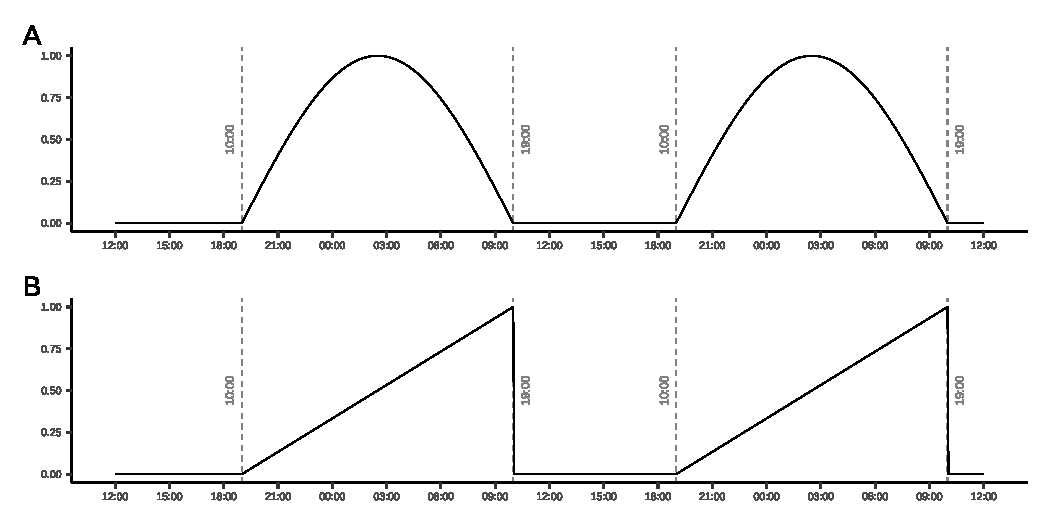
\includegraphics{visuals/sensor_independent.pdf}

}

\caption{\label{fig-sensor-independent}Sensor-independent features of
circadian rhythms across two consecutive nights. A) cosinus feature, B)
linear feature.}

\end{figure}

In addition to the engineered features, we chose to incorporate the
median-filtered raw predictions from the ZM device into our modeling
process. This decision stemmed from the understanding that children
typically undergo around five to eight sleep cycles per night, with
awakenings commonly occurring at the end of each
cycle\citep{galland_normal_2012}. Examining the raw ZM predictions, we
noted a significant overestimation in the number of awakenings per night
for the children in our study, exceeding what would be expected based on
typical sleep cycle patterns. Consequently, we elected to train and
evaluate our models using not only the raw ZM output, but also versions
that were subjected to 5-minute and 10-minute median filters. This
approach resulted in an anticipated, more age-appropriate count of
awakenings per night, providing a more accurate depiction of children's
sleep patterns (see Figure~\ref{fig-zm-median}).

\begin{figure}[b]

{\centering 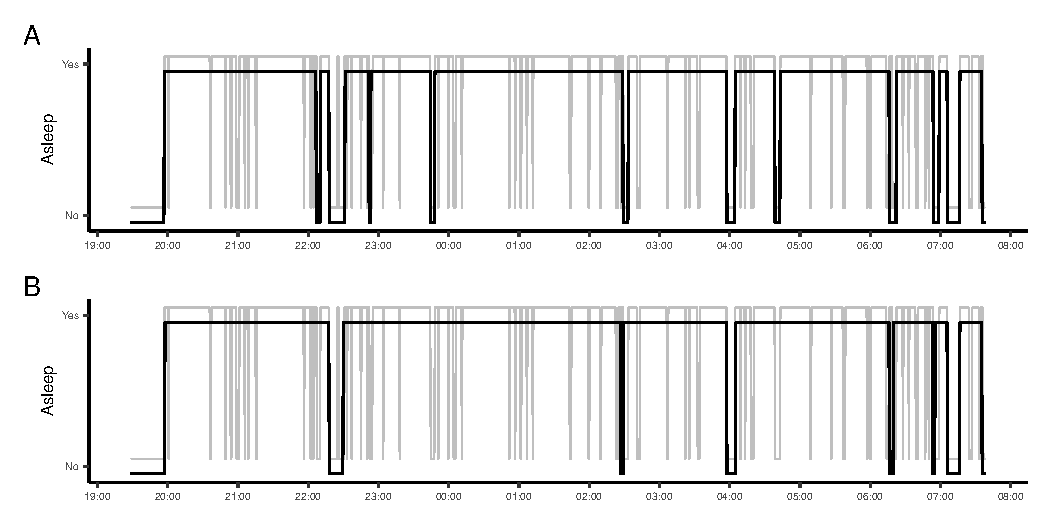
\includegraphics{visuals/zm_raw_vs_filtered.pdf}

}

\caption{\label{fig-zm-median}The difference in number of awakenings
between the raw ZM predictions vs.~5-minute, and 10-minute median
filtered predictions for a random night. Grey line is the raw
predictions, black line is the median filtered predictions. A: 5-minute
median filter on raw ZM predictions, B: 10-minute median filter on raw
ZM predictions.}

\end{figure}

\hypertarget{algorithms-training-and-validation}{%
\subsection{Algorithms, Training and
Validation}\label{algorithms-training-and-validation}}

In our study, we utilize two distinct modeling strategies to predict
sleep patterns derived from thigh-mounted accelerometer data: a
sequential ensemble and a multiclass bidirectional Long Short-Term
Memory (biLSTM)\citep{hochreiter1997} neural network. The sequential
ensemble involves using four pairs of models, each pair consisting of
the same algorithm, that predict in-bed and sleep time successively.
Conversely, the biLSTM is a comprehensive model that predicts multiple
classes simultaneously, effectively handling complex temporal patterns.
By applying and comparing both, we aim to evaluate their relative
effectiveness.

\hypertarget{models-in-sequence}{%
\subsubsection{Models in Sequence}\label{models-in-sequence}}

To predict in-bed time and sleep time accurately, we employed an
ensemble learning strategy based on sequential binary classification
models. This approach involved constructing a sequence of models using
multiple machine learning algorithms to improve predictive accuracy. The
process began with an initial model predicting in-bed time, followed by
a second model that utilized the output of the initial model to predict
sleep time. This sequential approach was applied across all four
algorithms detailed below, with each subsequent model leveraging the
outputs of the previous models for improved predictions.

\begin{enumerate}
\def\labelenumi{\arabic{enumi}.}
\item
  Logistic Regression (LREG): Logistic regression served as a simple and
  fast baseline model. However, due to its linear nature, it may
  struggle with capturing complex relationships and non-linear patterns
  present in the accelerometer data.
\item
  Decision Tree (TREE): Decision trees are capable of handling
  non-linear patterns and are easily interpretable. However, they are
  prone to overfitting, particularly when dealing with complex patterns
  that require simultaneous consideration of multiple features.
\item
  Single-layer Feed-forward Neural Network (SNN): Single-layer
  feed-forward neural networks can effectively capture non-linear
  relationships, even with their relatively simple structure. However,
  they tend to be more challenging to interpret compared to simpler
  models. Additionally, careful tuning of the network's architecture and
  training process is required to mitigate the risk of overfitting.
\item
  XGBoost (XGB): XGBoost is a powerful algorithm known for its ability
  to provide highly accurate predictions and handle complex, non-linear
  patterns in the data. It also incorporates built-in methods to prevent
  overfitting. However, training XGBoost models can be computationally
  intensive, and interpreting the predictions it generates can pose
  challenges.
\end{enumerate}

\hypertarget{multiclass-model}{%
\subsubsection{Multiclass Model}\label{multiclass-model}}

The biLSTM is a multiclass classifier capable of predicting the classes
of out-bed-awake, in-bed-awake, and in-bed-asleep. The architecture of
the biLSTM consisted of four layers, each with 128 hidden units. The
choice of four layers and 128 hidden units in our model balanced
complexity and efficiency: it was deep enough to learn intricate
patterns yet feasible to train timely. Additionally, the bidirectional
nature of the LSTM, doubling the hidden units at each time step,
improved data comprehension and avoided overfitting.

something on sequence length and step size

The biLSTM model was chosen for sleep classification using accelerometer
data from a thigh-mounted device due to its advantages in modeling
temporal context, handling a large temporal scope, and enabling temporal
inference over any feature without the need for hand-designed temporal
features.

Previous studies have explored the use of LSTM models for sleep
detection, showing promising results in capturing complex temporal
patterns. Notable works by Sano et al. \citep{sano2019} and Chen et al.
\citep{chen2021} have demonstrated the potential of LSTM models in
improving sleep detection based on accelerometer data. However, further
research is necessary to fully comprehend the strengths and limitations
of this approach.

\hypertarget{model-training}{%
\subsubsection{Model Training}\label{model-training}}

For the models in sequence, we trained four pairs of classification
models, each pair distinguishing between in-bed/out-of-bed and
asleep/awake states. The dataset was randomly split into a training set
(approximately 50\% of the subjects) and a testing set (also
approximately 50\%), ensuring that samples from the same subject were
never simultaneously used in both sets. Hyper-parameter optimization was
performed using 10-fold Monte Carlo cross-validation, with the F1 score
as the performance metric. The best-performing set of hyperparameters
was then used to fit the models to the full training dataset, maximizing
accuracy by leveraging all available data. Furthermore, the dataset for
predicting sleep was highly imbalanced which can pose challenges when
training machine learning models, as models may favor predicting the
majority class. To address this issue, we employed oversampling
techniques to ensure that each class had a roughly equal number of
training samples. Specifically, we utilized the Synthetic Minority
Over-sampling Technique (SMOTE)\citep{chawla2002}, which generates new
samples by interpolating random samples with their nearest neighbors. In
our study, we implemented SMOTE using the themis R
package\citep{themis}, resampling all classes to achieve a balanced
distribution of training samples.

The biLSTM model was trained using the Adam optimizer, which is
computationally efficient and adapts the learning rate during training.
Cross-entropy loss function was employed for its suitability in
multiclass classification with mutually exclusive classes. The softmax
activation function was selected for the output layer to obtain a
probability distribution over the classes. Data for training the biLSTM
were randomly divided into a training, validation, and test tensors
based on a 50/25/25 split. The model was evaluated using the F1 score on
both the training and validation sets. Early stopping was implemented
with a patience of 3 epochs, meaning training would stop if there was no
improvement in the validation loss for 3 consecutive epochs.

\hypertarget{model-validation-evt.-bare-statistics}{%
\subsubsection{Model Validation {[}evt. bare
``statistics''{]}}\label{model-validation-evt.-bare-statistics}}

In our study, we utilized standard evaluation metrics to assess the
performance of each model on an epoch-to-epoch basis. These include
accuracy (\(accuracy = \frac{TP+TN}{TP+TN+FP+FN}\)), sensitivity
(\(sensitivity = \frac{TP}{TP+FN}\)), specificity
(\(specificity = \frac{TN}{TN+FP}\)), precision
(\(precision = \frac{TP}{TP+FP}\)), negative predictive value (NPV,
\(NPV = \frac{TN}{TN + FN}\)), and F1 score
(\(F_1 = 2 * \frac{precision * sensitivity}{precision + sensitivity}\)).

In the context of our sequential learning strategy, the initial models
were tasked with the binary classification of in-bed vs.~out-of-bed. For
this task, we assessed performance using the F1-score, accuracy,
sensitivity, specificity, and precision metrics. The second models in
our sequential learning strategy focused on the binary classification of
asleep vs.~awake. For these models, we considered the same metrics, in
addition to the negative predictive rate. The class imbalance in this
case led us to compute the F1 score as an unweighted macro-average.
Additionally, we evaluated the multiclass classifier, biLSTM, using
macro-averaged F1-score, sensitivity, and precision. Furthermore, we
present precision-recall curves and receiver operating characteristic
curves, including the area under the curve, for each model and for each
type of ZM prediction.We considered both the in-bed/out-of-bed and
awake/asleep scoring tasks as binary classification problems,
designating in-bed and asleep as the positive labels and out-of-bed and
awake as the negative labels in accordance with previous
research\citep{hjorth2012, kushida2001}.

To evaluate our developed models' performance in assessing sleep quality
metrics, we employed Bland-Altman plots and Pearson correlations. These
methods were used to compare the sleep quality summaries calculated by
our models with those obtained from EEG-based ZM sleep quality
summaries. The sleep quality summaries included several metrics:

\begin{enumerate}
\def\labelenumi{\arabic{enumi}.}
\item
  Sleep Period Time (SPT) - This refers to the total duration of the
  sleep period, which is defined as the time from the start to the end
  of the ZM recording.
\item
  Total Sleep Time (TST) - This is the time spent asleep within the SPT.
\item
  Sleep Efficiency (SE) - This is the ratio between TST and SPT,
  representing the proportion of the sleep period that was actually
  spent asleep.
\item
  Latency Until Persistent Sleep (LPS) - This metric represents the time
  it takes to transition from wakefulness to sustained sleep. It is
  calculated as the time from the beginning of the ZM recording until a
  period when 10 out of 12 minutes are scored as sleep.
\item
  Wake After Sleep Onset (WASO) - This refers to the time spent awake
  after initially falling asleep and before the final awakening. In our
  analysis, a period is counted as `awake' only if it consists of 3 or
  more contiguous 30-second epochs which is also how the ZM summarizes
  WASO.
\end{enumerate}

R version 4.3.0 (2023-04-21)\citep{R-lang} and the
Tidymodels\citep{tidymodels} and Tidyverse\citep{tidyverse} suite of
packages were used as the core tools for model development and analyses.
Python version 3.10.6\citep{10.5555/1593511} and
PyTorch\citep{NEURIPS2019_9015} were used to implement the biLSTM model.
All code used to perform the analysis and generate the figures in this
paper are available in
\href{https://github.com/esbenlykke/sleep_study}{this repository}.

\hypertarget{results}{%
\section{Results}\label{results}}

\begin{figure}[b]

{\centering 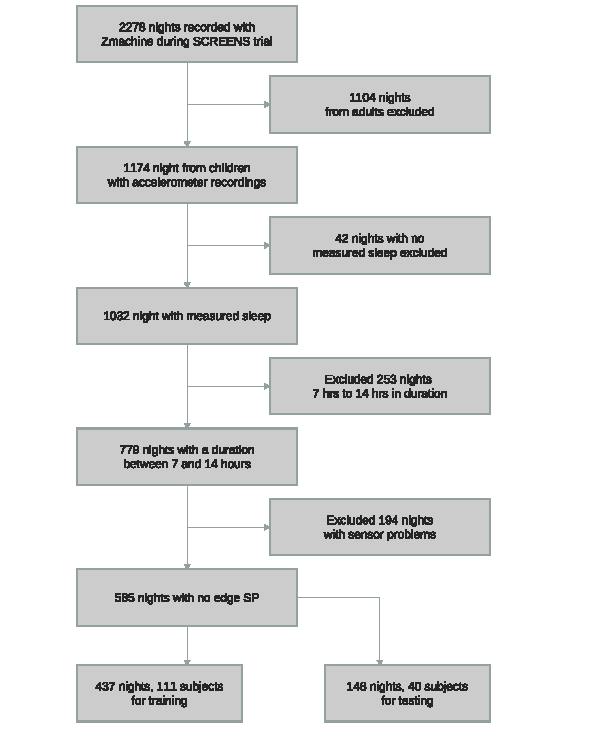
\includegraphics{visuals/flowchart_of_elligible_nights.pdf}

}

\caption{Flowchart of eligible nights included in the study - revise
text boxes!}

\end{figure}

The analysis included children with an average age of 9.4 years (SD =
2.1). The raw ZM predictions covered 2,035,261 sleep epochs, or about
86\% of the total recording duration.

As reported in Table~\ref{tbl-zm_overview} the sleep quality metrics
derived from ZM predictions were modified by the implementation of
5-minute and 10-minute median filters. The Sleep Period Time (SPT) were
consistent across raw and filtered datasets (mean: 9.2 ± 2.1 hours) as
this corresponds to the length of the ZM recording. Total Sleep Time
(TST) and Sleep Efficiency (SE) increased in the filtered data, implying
the filters categorize some wakefulness as sleep. Specifically, TST
increased from a raw mean of 7.7 ± 1.9 hours to 8.1 ± 2.0 hours
(5-minute filter) and 8.2 ± 2.1 hours (10-minute filter), while SE rose
from 82.6 ± 12.0\% to 86.4 ± 12.7\% and 87.5 ± 12.9\% respectively.
Latency to Persistent Sleep (LPS) also elevated, suggesting the filter
smooths out brief awakenings at sleep onset, leading to a prolonged time
to persistent sleep. The most significant change was seen in Wake After
Sleep Onset (WASO), which dropped from 39.0 ± 33.6 minutes in raw data
to 30.6 ± 46.8 minutes and 22.3 ± 55.4 minutes in the 5-minute and
10-minute filtered data, respectively. The number of awakenings was also
considerably reduced with the application of filters. In the raw data,
the average number of awakenings was 34.46 ± 11.33 per night, which
reduced to 4.43 ± 3.26 and 1.95 ± 2.01 for the 5-minute and 10-minute
filtered data sets respectively. These results underscore the role of
median filters on sleep metrics.

\hypertarget{tbl-zm_overview}{}
\begin{longtable}{lrrrrrr}
\caption{\label{tbl-zm_overview}Overview of characteristics of the ZM sleep quality summaries per night.
Values are represented as mean (SD). }\tabularnewline

\toprule
 & SPT (hrs) & TST (hrs) & SE (\%) & LPS (min) & WASO (min) & Awakenings (N) \\ 
\midrule
Raw ZM Predictions & 9.21 (2.15) & 7.74 (1.93) & 82.61 (11.97) & 34.53 (27.87) & 39 (33.56) & 34.46 (11.33) \\ 
5-Min Median & 9.21 (2.15) & 8.1 (2.03) & 86.35 (12.72) & 36.26 (39.8) & 30.63 (46.84) & 4.43 (3.26) \\ 
10-Min Median & 9.21 (2.15) & 8.21 (2.06) & 87.54 (12.89) & 37.99 (48.7) & 22.27 (55.38) & 1.95 (2.01) \\ 
\bottomrule
\end{longtable}

\hypertarget{performance-on-epoch-to-epoch-basis}{%
\subsection{Performance on Epoch-To-Epoch
Basis}\label{performance-on-epoch-to-epoch-basis}}

The epoch-to-epoch evaluation of in-bed performance metrics, outlined in
Table~\ref{tbl-in_bed_performance}, demonstrates practically equivalent
performance across all model types. While the Decision Tree model posted
an F1 score of 94.4\% and accuracy of 95.3\%, the Logistic Regression
and Feed-Forward Neural Network models each exhibited an F1 score of
95.0\% and similar accuracies of 95.7\% and 95.8\%, respectively. The
XGBoost model, despite recording the highest metrics with an F1 score of
95.4\% and accuracy of 96.1\%, outpaced the others only marginally. This
underscores the consistency of performance among these models in
classifying in-bed conditions.

\hypertarget{tbl-in_bed_performance}{}
\begin{longtable}{lrrrrr}
\caption{\label{tbl-in_bed_performance}In-Bed Performance Metrics }\tabularnewline

\toprule
 & F1 Score (\%) & Accuracy (\%) & Sensitivity (\%) & Precision (\%) & Specificity (\%) \\ 
\midrule
Decision Tree & $94.36$ & $95.27$ & $93.12$ & $95.64$ & $96.86$ \\ 
Logistic Regression & $94.99$ & $95.74$ & $95.03$ & $94.94$ & $96.26$ \\ 
Feed-Forward Neural Net & $95.03$ & $95.77$ & $95.07$ & $94.99$ & $96.29$ \\ 
XGBoost & $95.38$ & $96.06$ & $95.83$ & $94.94$ & $96.23$ \\ 
\bottomrule
\end{longtable}

Table~\ref{tbl-sleep_performance} details the performance of the
sequential models on raw and median-filtered (5 and 10 minute) ZM
predictions. The F1 Scores, which are unweighted macro averages, for raw
ZM predictions range from 71.05\% to 76.18\%. The models perform
comparably, but the low Specificity values (62.84\% to 70.93\%) suggest
difficulty in correctly classifying negative instances. Applying
5-minute median filtering improves the performance metrics. The XGBoost
model tops the charts with an F1 Score of 79.22\% and NPV of 74.00\%.
However, Specificity still remains low, with values between 54.68\% and
74.84\% across all models. With 10-minute median filtering, the metrics
improve further. The XGBoost model still leads with an F1 Score of
80.87\% and an NPV of 75.76\%. But, Specificity remains a concern,
ranging from 57.47\% to 76.35\% across all models.

\hypertarget{tbl-sleep_performance}{}
\begin{longtable}{cccccc}
\caption{\label{tbl-sleep_performance}Sleep Performance Metrics }\tabularnewline

\toprule
 & F1 Score (\%) & Precision (\%) & NPV (\%) & Sensitivity (\%) & Specificity (\%) \\ 
\midrule
\multicolumn{6}{l}{Raw ZM Predictions} \\ 
\midrule
Decision Tree & $72.94$ & $93.24$ & $48.36$ & $86.34$ & $67.15$ \\ 
Logistic Regression & $71.05$ & $93.72$ & $43.88$ & $82.72$ & $70.93$ \\ 
Neural Network & $71.76$ & $93.77$ & $45.13$ & $83.59$ & $70.83$ \\ 
XGBoost & $76.18$ & $92.80$ & $57.98$ & $91.32$ & $62.84$ \\ 
\midrule
\multicolumn{6}{l}{5-Min Median} \\ 
\midrule
Decision Tree & $75.48$ & $94.20$ & $55.46$ & $93.35$ & $59.01$ \\ 
Logistic Regression & $68.32$ & $95.84$ & $36.03$ & $81.36$ & $74.84$ \\ 
Neural Network & $71.74$ & $95.78$ & $41.64$ & $85.62$ & $73.11$ \\ 
XGBoost & $79.22$ & $93.87$ & $74.00$ & $97.30$ & $54.68$ \\ 
\midrule
\multicolumn{6}{l}{10-Min Median} \\ 
\midrule
Decision Tree & $76.28$ & $94.74$ & $58.06$ & $94.86$ & $57.47$ \\ 
Logistic Regression & $67.96$ & $96.54$ & $34.29$ & $81.87$ & $76.35$ \\ 
Neural Network & $70.95$ & $96.06$ & $39.54$ & $86.48$ & $71.37$ \\ 
XGBoost & $80.87$ & $94.90$ & $75.76$ & $97.72$ & $57.60$ \\ 
\bottomrule
\end{longtable}

The analysis of precision-recall and ROC curves across different models
and ZM prediction types shows varying performance. In terms of
precision-recall AUC, the Decision Tree model consistently outperforms
others, indicating its superior predictive accuracy (see
Figure~\ref{fig-pr_curves}). Conversely, the Neural Network model
generally shows weaker performance. However, for ROC AUC, the XGBoost
model consistently excels across all data types, indicating a strong
ability to differentiate between classes, while the Neural Network model
tends to underperform (see Figure~\ref{fig-roc_curves}). The F-measure
(F1 score) shows variable performance across different configurations
but generally, the Decision Tree model yields higher scores.

\begin{figure}[b]

{\centering 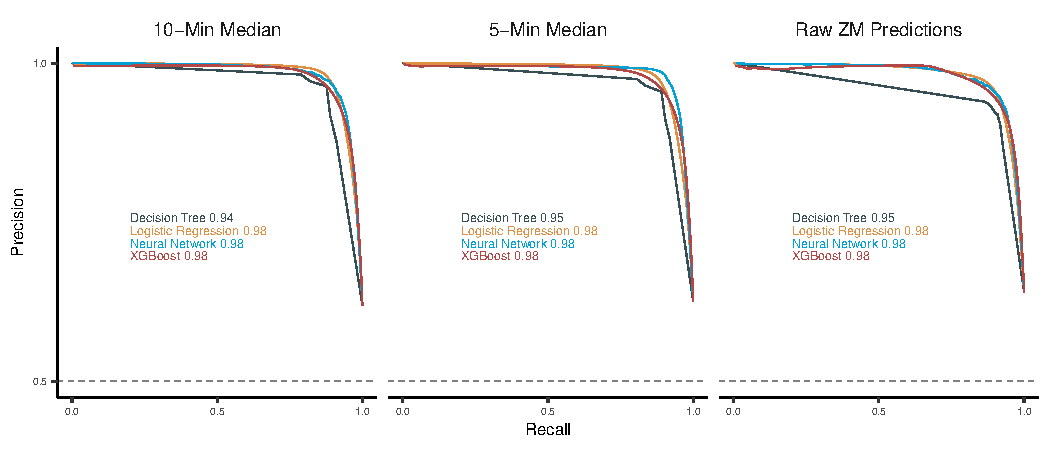
\includegraphics{visuals/plot_sleep_pr.pdf}

}

\caption{\label{fig-pr_curves}Precision-recall curves of the models
evaluated across the different ZM predictions, including raw ZM
predictions, as well as 5-minute and 10-minute median smoothing of the
ZM raw predictions. The x-axis of the plot represents the proportion of
true wake epochs that were correctly classified as wake, while the
y-axis represents the proportion of all epochs labeled as wake by the
classifier that were classified correctly. The area under the curve
values are displayed as color-coded text in the plot indicate the area
under the Precision-Recall curve for each model and condition.}

\end{figure}

\begin{figure}[b]

{\centering 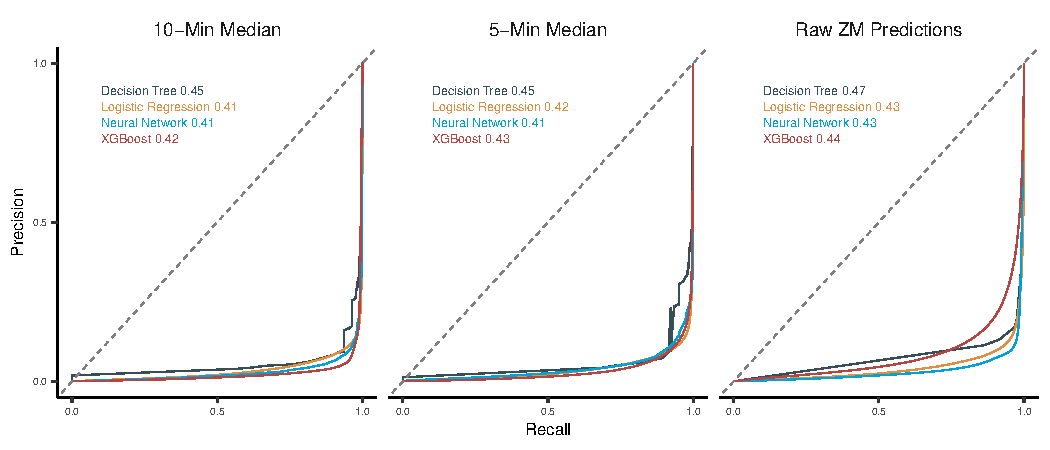
\includegraphics{visuals/plot_sleep_roc.pdf}

}

\caption{\label{fig-roc_curves}Receiver operating characteristic curves
of the models evaluated across the different ZM predictions, including
raw ZM predictions, as well as 5-minute and 10-minute median smoothing
of the ZM raw predictions. The x-axis of the plot represents the
proportion of true asleep epochs that were incorrectly classified as
awake, while the y-axis represents the proportion of all epochs labeled
as awake by the classifier that were correctly classified. The area
under the curve values displayed are displayed as color-coded text in
the plot to indicate the area under the receiver operating
characteristic curve for each model and condition.}

\end{figure}

Table~\ref{tbl-biLSTM_performance} presents the performance of the
three-class biLSTM multiclassifier on raw and median-filtered (5-minute
and 10-minute) ZM predictions. Raw ZM predictions achieve F1 Scores
ranging from 71.36\% to 76.04\%, indicating overall good performance.
Applying 5-minute median filtering improves the metrics further,
resulting in F1 Scores ranging from 75.99\% to 78.53\%, demonstrating
enhanced precision and sensitivity. However, Specificity values are not
available for this configuration. With 10-minute median filtering, F1
Scores range from 73.45\% to 73.93\%, maintaining good performance but
with limited information on Specificity. Further analysis is required to
assess performance across all classes.

\hypertarget{tbl-biLSTM_performance}{}
\begin{longtable}{cccc}
\caption{\label{tbl-biLSTM_performance}Performance of the three-class biLSTM multicclassifier. }\tabularnewline

\toprule
 & F1 Score & Sensitivity & Precision \\ 
\midrule
Raw ZM Predictions & $71.36$ & $70.42$ & $76.04$ \\ 
5-Min Median & $75.99$ & $74.62$ & $78.53$ \\ 
10-Min Median & $73.45$ & $73.93$ & $73.07$ \\ 
\bottomrule
\end{longtable}

\hypertarget{evaluation-of-sleep-quality-summaries}{%
\subsection{Evaluation of Sleep Quality
Summaries}\label{evaluation-of-sleep-quality-summaries}}

BA plots

pearson regression

scatterplots with identity line and best linear fit

\newpage


\renewcommand\refname{References}
  \bibliography{bibliography.bib}


\end{document}
